\documentclass[amsmath,amssymb,notitlepage,12pt]{revtex4-1}
\usepackage{graphicx}
\usepackage{bm}% bold math
\usepackage{multirow}
\usepackage{booktabs}
\usepackage{verbatim}
\usepackage{hyperref}
\hypersetup{pdftex,colorlinks=true,allcolors=blue}
\usepackage{hypcap}
%\usepackage[small,compact]{titlesec}
%\usepackage{showkeys}
%\addtolength{\textheight}{0.3cm}
%\addtolength{\topmargin}{-0.15cm}
%\addtolength{\textwidth}{0.4cm}
%\addtolength{\hoffset}{-0.2cm}
\begin{document}
\hspace*{11.5cm}CLAS-NOTE 2013-008

\title{RTPC Alignment Calibration for EG6}%\\Version 0.1}
\author{N. Baltzell}
\affiliation{Argonne National Laboratory}
\date{\today}
\begin{abstract}
The position of the Radial Time Projection Chamber relative to EG6's 1.206 GeV beamline is measured with elastic scattering to be $x=-0.28$ mm, $y=-0.97$ mm.
\end{abstract}
\maketitle
%\tableofcontents

\section{Introduction}
%Recoil nuclei are measured in the RTPC's drift region only a few cm from the beamline.
Due to its small size, proximity to the beamline, and beamline constraint in track fitting, the RTPC is sensitive to radial misalignment as small as a few-hundred $\mu$m.  Unless accounted for, this results in errors on momentum reconstruction that modulate systematically with the azimuth around the detector.
%At the kinematics of elastic recoils in EG6's 1.206 GeV data, the effect is a modulation with amplitude of 10\% in momentum and 2.5$^\circ$ in $\phi$ per mm of misalignment.

Measuring a misalignment requires a reference.  The higher energy tracks in CLAS leave only small signals in the RTPC, and the two detectors have small overlap in acceptance.  Instead of measuring the same track in both detectors, elastic scattering is used with the electron measured in CLAS and the $^4$He in the RTPC.  This same event selection has also been the source of drift paths and gain calibrations \cite{driftpaths,gains}, which have proven sensitive to alignment.

The method described here
%to measure the beam position relative to the RTPC
is similar to that for measuring the beam position relative to CLAS \cite{clasbeamoffset} in that misalignment results in a modulation of a reconstructed quantity as a function of $\phi$.  In the latter case, the beam window is the reference and the $z$-vertex reconstructed by CLAS is what modulates, while here it is CLAS's electron that serves as a reference and the RTPC's measured $\phi$ and momentum that modulate. 

\section{Motivation}\label{sec:motivation}
The beamline constraint in RTPC reconstruction takes the form of one additional point in the helix fit with zero weight on its $z$-coordinate.  The effect of this constraint was investigated by varying its $(x_0,y_0)$ position and refitting each track.  For tracks at average elastic kinematics, the effect on reconstructed momentum and $\phi$ is shown in Fig. \ref{fig:example_phi} for four different beamline offsets.   At these kinematics there is 20\% variation in momentum and 5$^\circ$ variation in $\phi$ per mm of offset but no significant effect on $\theta$ nor $z$-vertex.%. there is no significant effect on $z$-vertex and $\theta$, but there is 20\% variation in momentum and 5$^\circ$ variation in $\phi$ from a 1 mm offset.
%The particlar value of $(1.55$mm$,0.29$mm$)$ is included in Fig. \ref{fig:example_phi} because it was measured in \cite{clasbeamoffset} and then incorrectly used as the beam position relative to the RTPC/RTPC relative alignment, when that was really a measurement of beam/CLAS alignment.

\begin{figure}[btp]\centering
    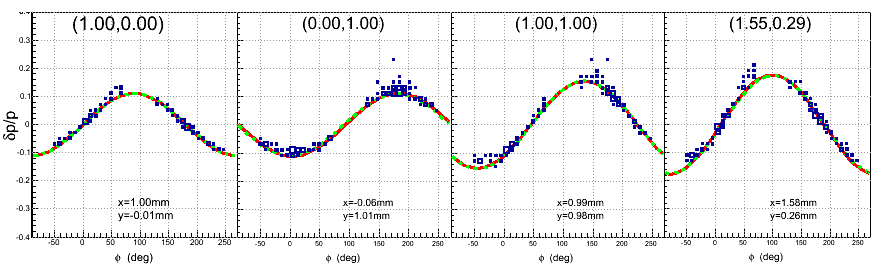
\includegraphics[width=16cm]{pics/offsets_phi}
    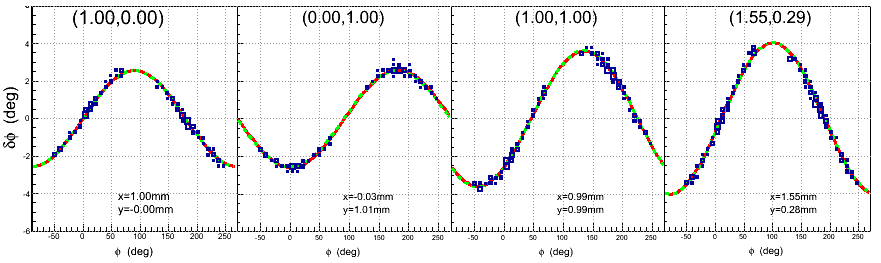
\includegraphics[width=16cm]{pics/offsets_mom}
    \caption{The effect on reconstructed momentum (top) and $\phi$ (bottom) as a function of the track's $\phi$ of moving the beamline constraint from $(0,0)$ to the position $(x_0,y_0)$, shown at the top of each figure in mm.  The data are for tracks with $p/q\sim125$ MeV and $\theta\sim78^\circ$.\label{fig:example_phi}}
\end{figure}

The following equations, with amplitude and phase related to the beam position $(x_0,y_0)$ relative to the RTPC's axis, are sufficient to describe the effects near elastic kinematics.%  The variable $\phi$ is the azimuthal angle of the RTPC track.
\begin{equation}
    \Delta\phi = \left[\frac{2.56^\circ}{mm}\right] \Bigl(-y_0 \cos\phi + x_0 \sin\phi\Bigr)
    \label{eq:phi}
\end{equation}
\begin{equation}
    \frac{\Delta p}{p} = \left[\frac{p\sin\theta}{1078\ MeV\cdot mm}\right] \Bigl(-y_0 \cos\phi + x_0 \sin\phi\Bigr)
    \label{eq:mom}
\end{equation}
The red curves in Fig. \ref{fig:example_phi} are the results of fitting with these functions, and the values at the bottom of each plot are the fit parameters after minimization and reproduce well the expected values.

For large momentum or small $\theta$ this parameterization starts to fail.  While it should be possible in the future to find a global function that applies over all kinematics as an ad-hoc momentum correction after the raw data have been processed, it is desireable to determine the correct beam position for the purpose of drift-path and gain calibrations and also to minimize future corrections.

\section{Method}\label{sec:method}
In order to apply the idea of Section \ref{sec:motivation}, it is neccessary to measure a modulation in the RTPC by comparing with a reference.  Elastic scattering provides a correlated electron measured in CLAS suited for this purpose, assuming it is well-measured and has no $\phi$-oscillation of its own due also to tracking to the wrong beam position in the solenoid field.  Selection of elastically scattered electrons and $^4$He was studied previously for EG6 and the same event selection is used here \cite{driftpaths,gains}. 

In fact, the EG1b run also had the solenoid target field (without the RTPC) but with a beam rastered over a 1.5 cm diameter target, and corrections were developed to account for CLAS reconstruction effects due to beam position \cite{eg1braster}.  Assuming the same effect for EG6 and accounting for our 21\% smaller solenoid field, combined with the fact that the 
EG6 beam position is measured to be $\sim$1.6 mm from CLAS's $z$-axis in the 1.206 GeV data \cite{clasbeamoffset}, we can then expect an average modulation of $\phi$ of $\sim$0.3$^\circ$ for the elastic electrons in this analysis.  This is repesented by the red line in Fig. \ref{fig:dphi_vs_z}.

\begin{figure}[hbtp]\centering
%    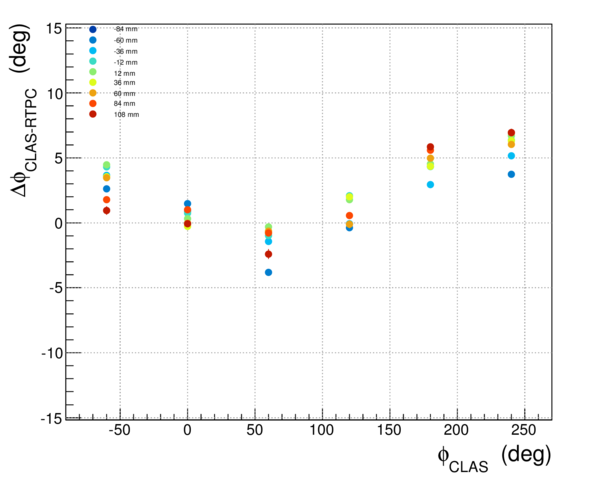
\includegraphics[width=8cm]{pics/dphi_z_v9}
    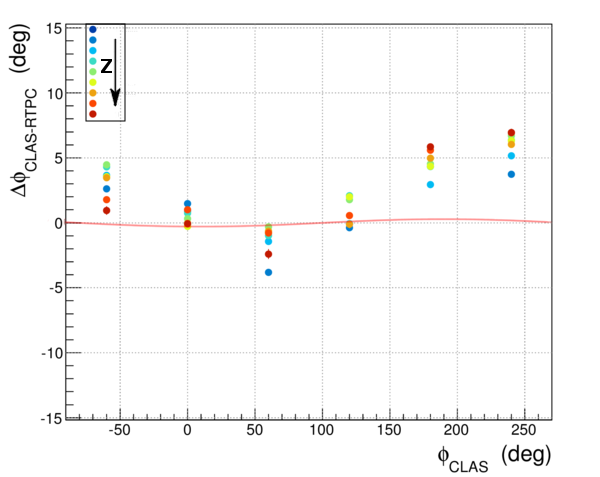
\includegraphics[width=8cm]{pics/dphi_z_v9_plus_bosted}
    \caption{The difference between $\phi$ reconstructed from CLAS's electron and RTPC's $^4$He for elastic scattering ($y$-axis is shifted by $180^\circ$).  Colors correspond to $z$-vertex positions over the 20 cm range of the RTPC.  The curve represents the expected contribution from the electron by extrapolating EG1b corrections to EG6 conditions.\label{fig:dphi_vs_z}}
\end{figure}
It is also noteworthy that EG6's $\Delta\phi$ between CLAS and RTPC for elastics has little dependence on $z$-vertex, while the electrons have traveled through much different solenoid $\int\vec{B}\cdot \vec{dl}$ for different $z$.
Using the electron's $\phi$ measured by CLAS as a reference, the $3.5^\circ$ $\Delta\phi_{CLAS-RTPC}$ oscillation in Fig. \ref{fig:dphi_vs_z} is then attributed entirely to RTPC misalignment.  By fitting with Eq. \ref{eq:phi}, the beam position relative to the RTPC can be extracted.


\section{Results}

The left panel in Fig. \ref{fig:dphi_CLAS} shows the oscillation fit using Eq. \ref{eq:phi} and the resulting beam offset in the first two fit parameters.  However, those RTPC tracks were reconstructed with an incorrect beam offset, and adjusting for that results in a current best estimate of the beam position of $(x_0,y_0)=(0.28$ mm$,0.97$ mm$)$ relative to the RTPC.  
After refitting the elastic $^4$He tracks with this new beam position, the result is as expected in the right plot of Fig. \ref{fig:dphi_CLAS}:  the modulation is removed.  The overall $2.4^\circ$ shift is the result of recalibrating the drift paths with this new beam offset.

\begin{figure}[htbp]\centering
    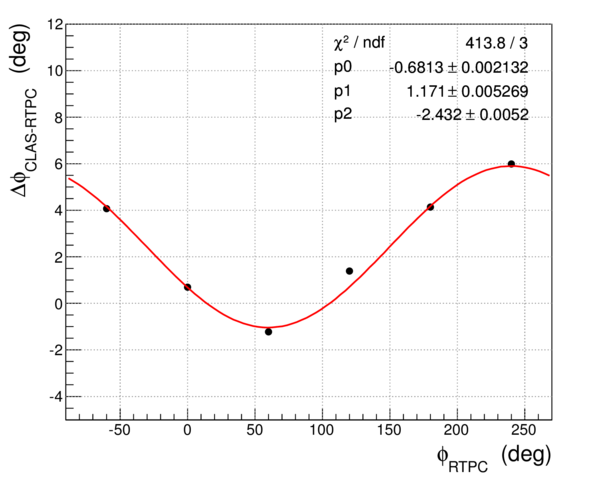
\includegraphics[width=8cm]{pics/CLASRTPC_dphi_phi_epass1v9.png}
    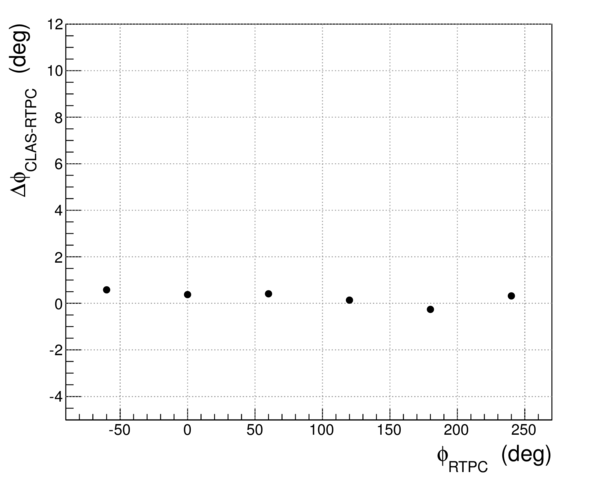
\includegraphics[width=8cm]{pics/Elasticdphi_vsphi_v11.png}
    \caption{The difference between $\phi$ reconstructed from CLAS's electron and RTPC's $^4$He for elastic scattering for two different beam offsets relative to the RTPC axis: $(1.55$ mm, $0.29$ mm$)$ on left and $(0.28$ mm, $0.97$ mm$)$ on right.
    \label{fig:dphi_CLAS}}
\end{figure}

%If the target is aligned in the center of the RTPC, then the measured beam position is 1 mm from the center of the target.  The radius of the EG6 target is 6 mm, and upstream is a support structure of only 5 mm diameter.  However, this is still reasonable as the beam width is only a couple hundred $\mu$m.

Independent confirmation of this method is provided by the effect on momentum, which from Fig. \ref{fig:example_phi} and Eq. \ref{eq:mom} is expected to be significant for an offset of this size.  The elastic $^4$He momentum had previously been shifted by well over 10\% in one half of the RTPC relative to the other.  After using the corrected beam position, the momentum distributions are much more symmetric as shown in the right panel of Fig. \ref{fig:dp_CLAS}.

\begin{figure}[htbp]\centering
    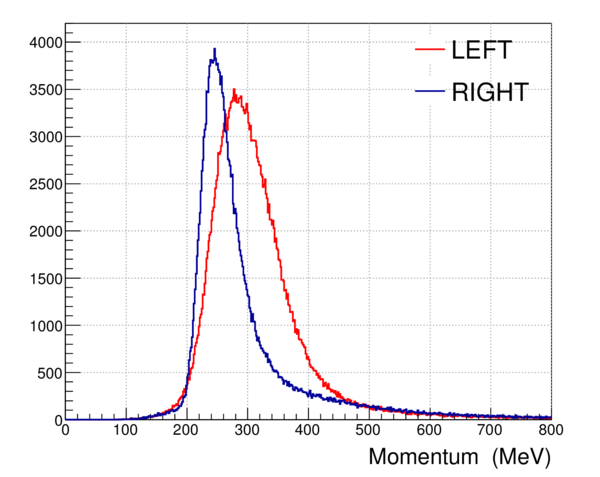
\includegraphics[width=8cm]{pics/CLASRTPC_dp_phi_epass1v9_precorr.png}
    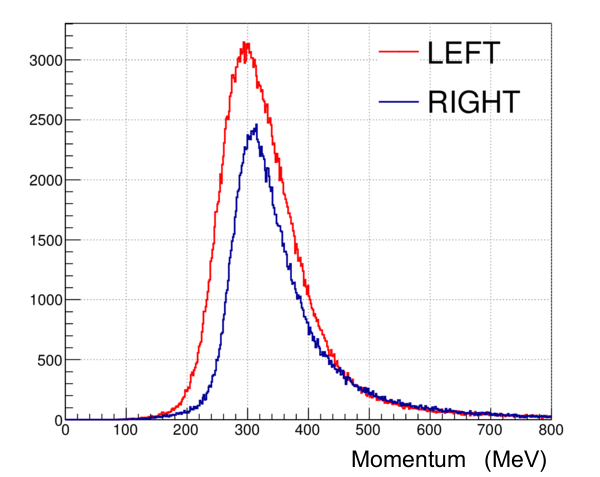
\includegraphics[width=8cm]{pics/Elasticmom_v11_2.png}
    \caption{The momentum distributions for elastic $^4$He measured by the two halves of the RTPC (LEFT/RIGHT in the legend) before (left) and after (right) the alignment calibration.\label{fig:dp_CLAS}}
\end{figure}




\bibliography{tpcalign}
\end{document}

